%%%%%%%%%%%%%%%%%%%%%%%%%%%%%%%%%%%%%%%%%
% University/School Laboratory Report
% LaTeX Template
% Version 3.0 (4/2/13)
%
% This template has been downloaded from:
% http://www.LaTeXTemplates.com
%
% Original author:
% Linux and Unix Users Group at Virginia Tech Wiki 
% (https://vtluug.org/wiki/Example_LaTeX_chem_lab_report)
%
% License:
% CC BY-NC-SA 3.0 (http://creativecommons.org/licenses/by-nc-sa/3.0/)
%
%%%%%%%%%%%%%%%%%%%%%%%%%%%%%%%%%%%%%%%%%

%----------------------------------------------------------------------------------------
%	PACKAGES AND DOCUMENT CONFIGURATIONS
%----------------------------------------------------------------------------------------

\documentclass{article}

\usepackage[version=3]{mhchem} % Package for chemical equation typesetting
\usepackage{siunitx} % Provides the \SI{}{} command for typesetting SI units

\usepackage{graphicx}
\usepackage{caption}
\usepackage{subcaption}
\usepackage{cancel}

\usepackage{float}

\usepackage[T1]{fontenc} % allow small bold caps

\usepackage{listings}
\usepackage{color}

\definecolor{dkgreen}{rgb}{0,0.6,0}
\definecolor{gray}{rgb}{0.5,0.5,0.5}
\definecolor{mauve}{rgb}{0.58,0,0.82}

\lstset{frame=tb,
  language=Matlab,
  aboveskip=2mm,
  belowskip=2mm,
  showstringspaces=false,
  columns=flexible,
  basicstyle={\small\ttfamily},
  numbers=none,
  numberstyle=\tiny\color{gray},
  keywordstyle=\color{blue},
  commentstyle=\color{dkgreen},
  stringstyle=\color{mauve},
  breaklines=true,
  breakatwhitespace=true
  tabsize=2
}

\setlength\parindent{0pt} % Removes all indentation from paragraphs

\renewcommand{\labelenumi}{\alph{enumi}.} % Make numbering in the enumerate environment by letter rather than number (e.g. section 6)

\usepackage[margin=1in]{geometry}

\usepackage{amssymb}


%\usepackage{times} % Uncomment to use the Times New Roman font

%----------------------------------------------------------------------------------------
%	Title
%----------------------------------------------------------------------------------------

\begin{document}
\pagenumbering{gobble}

\title{6.s02: EECS II - From A Medical Perspective}
\author{
  Ryan Lacey <rlacey@mit.edu>\\
  \footnotesize \texttt{Collaborator(s): None}
}
        
\maketitle
        

\begin{enumerate}
\item[1.]
	\begin{enumerate}
	\item[(a)]
		$\;$\\ 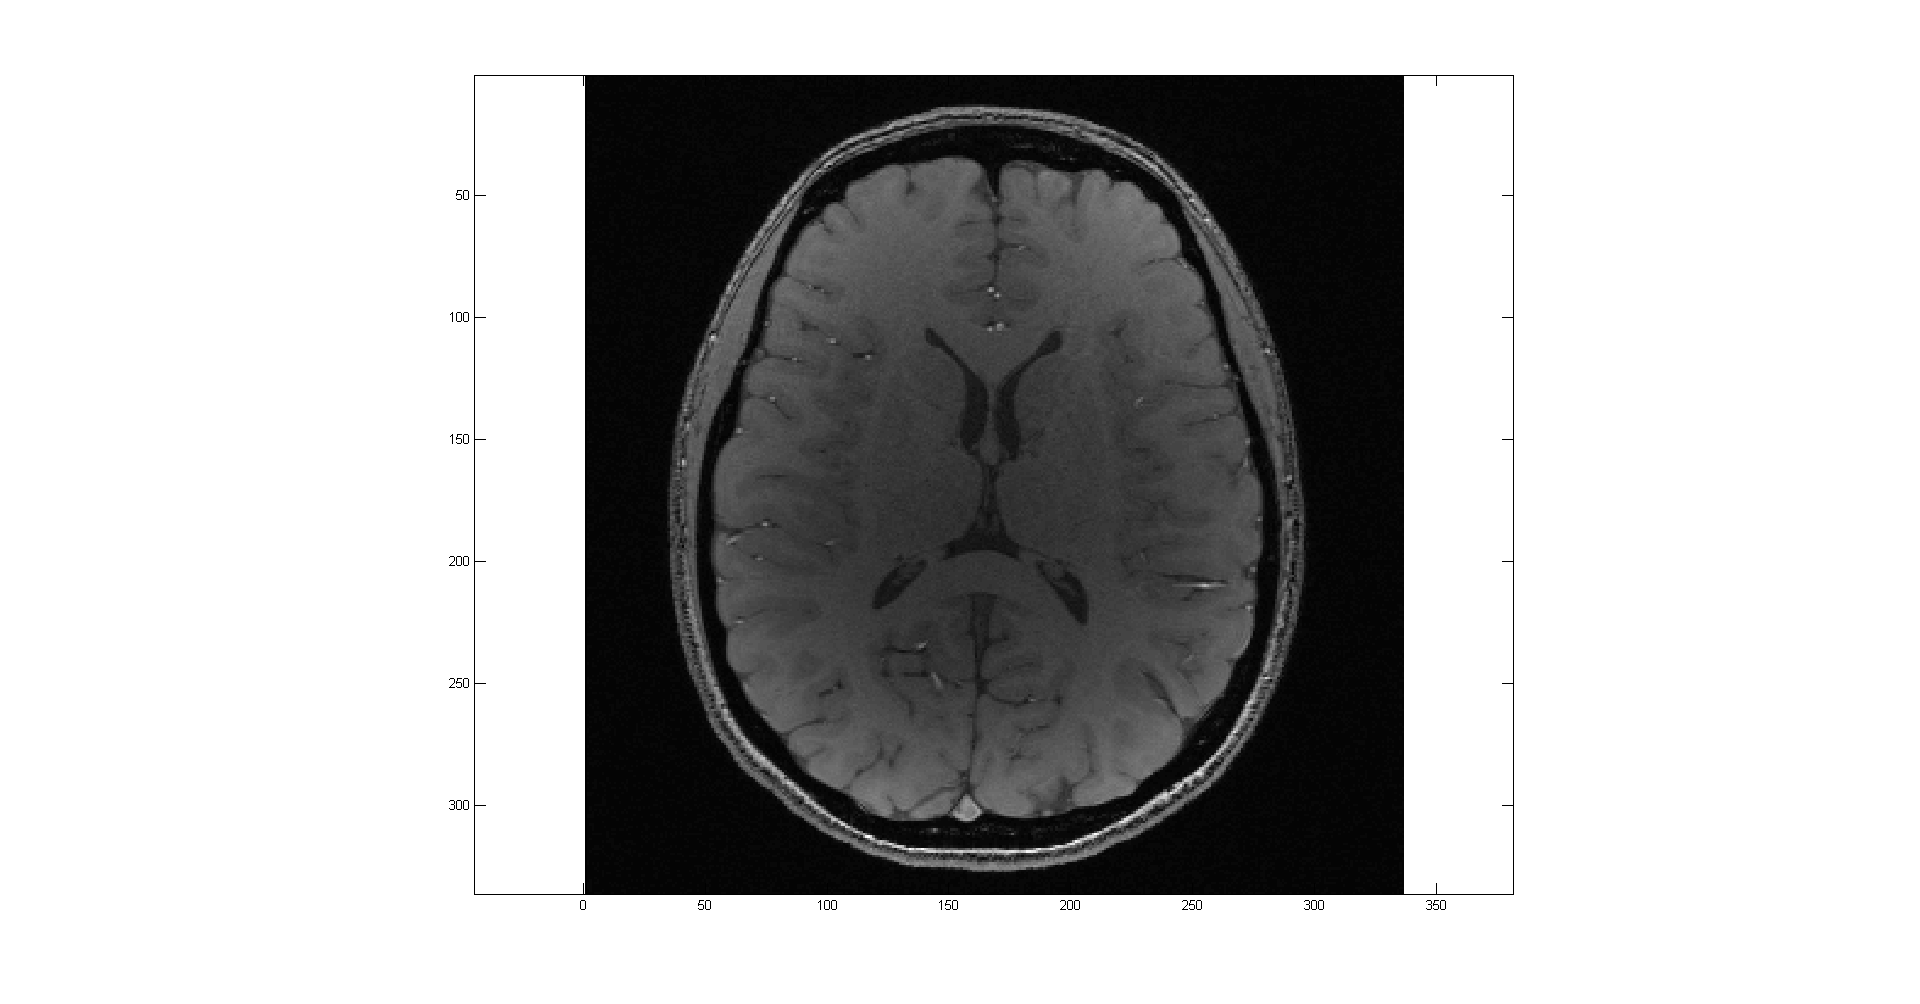
\includegraphics[width=\textwidth]{../images/GrayscaleBrain} \\
\begin{lstlisting}   
brain = kspace2image(kspace); 
imagesc(abs(brain));
\end{lstlisting}

\bigskip
\bigskip

	\item[(b)]
	PLACE\\

\newpage

	\item[(c)]
		$\;$\\ 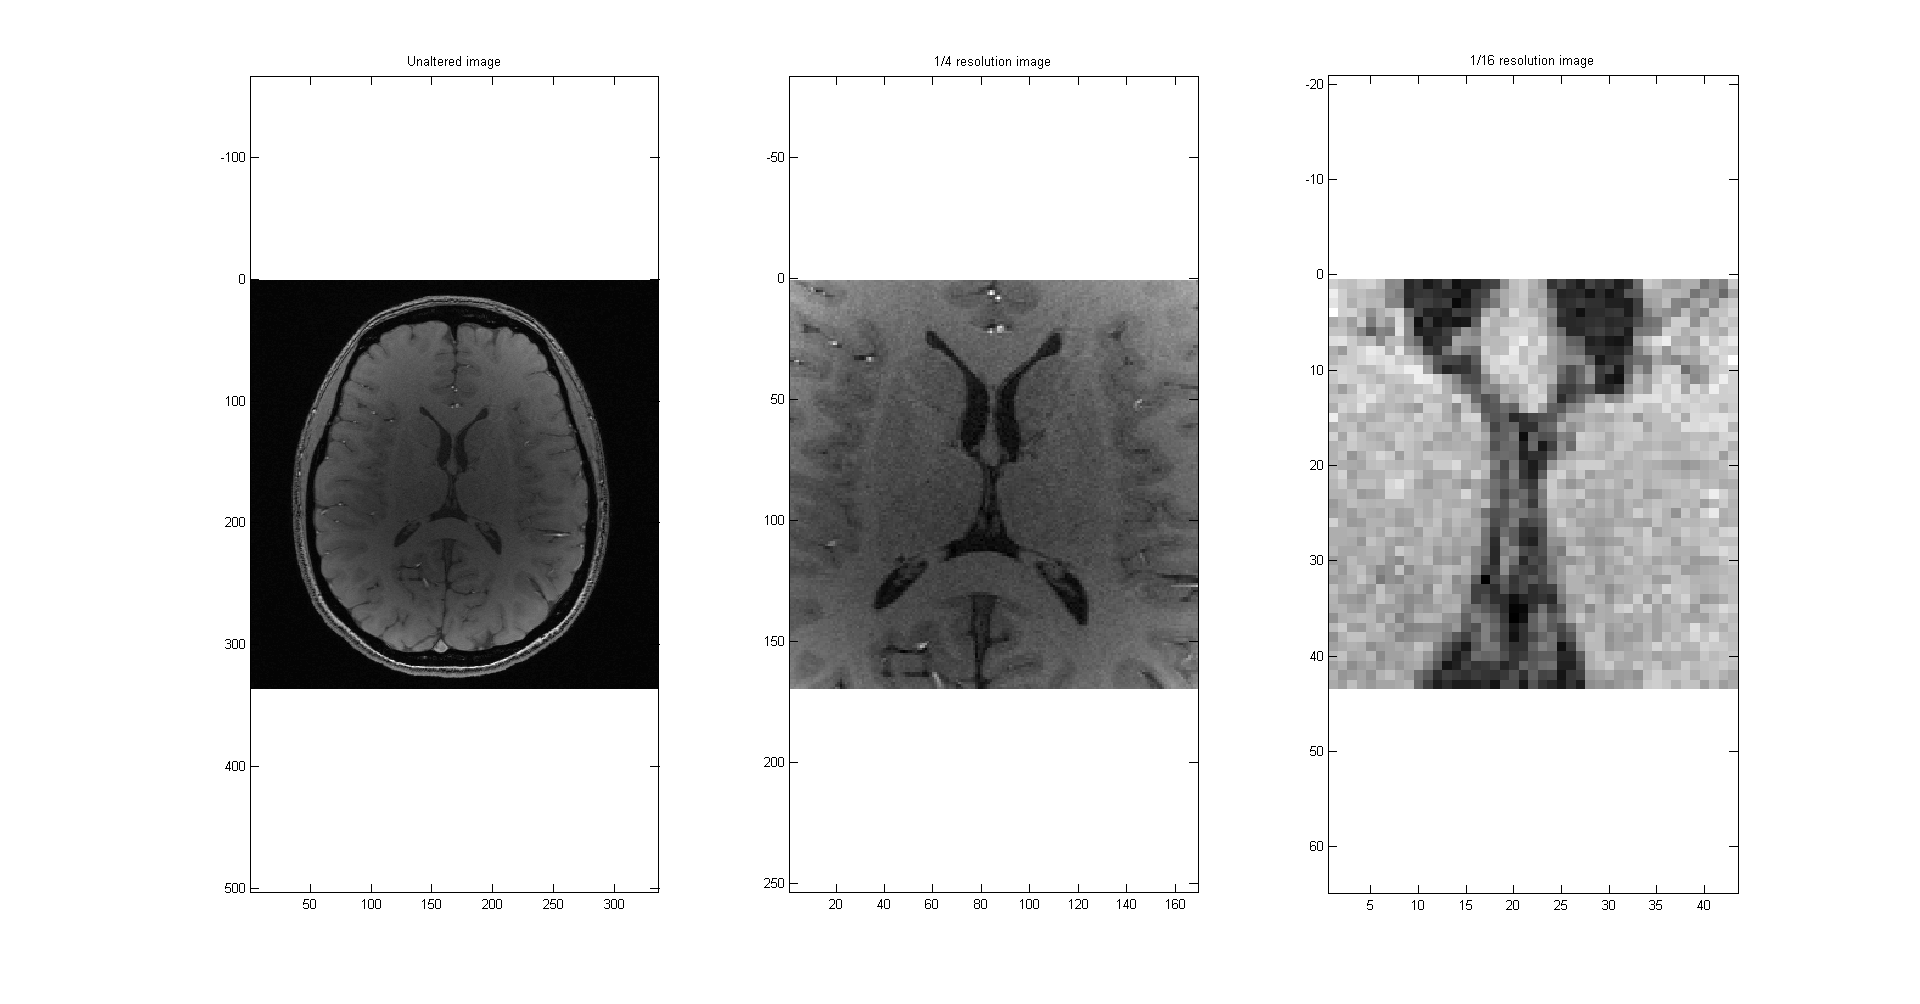
\includegraphics[width=\textwidth]{../images/BrainResolutions} \\
		$\;$\\ 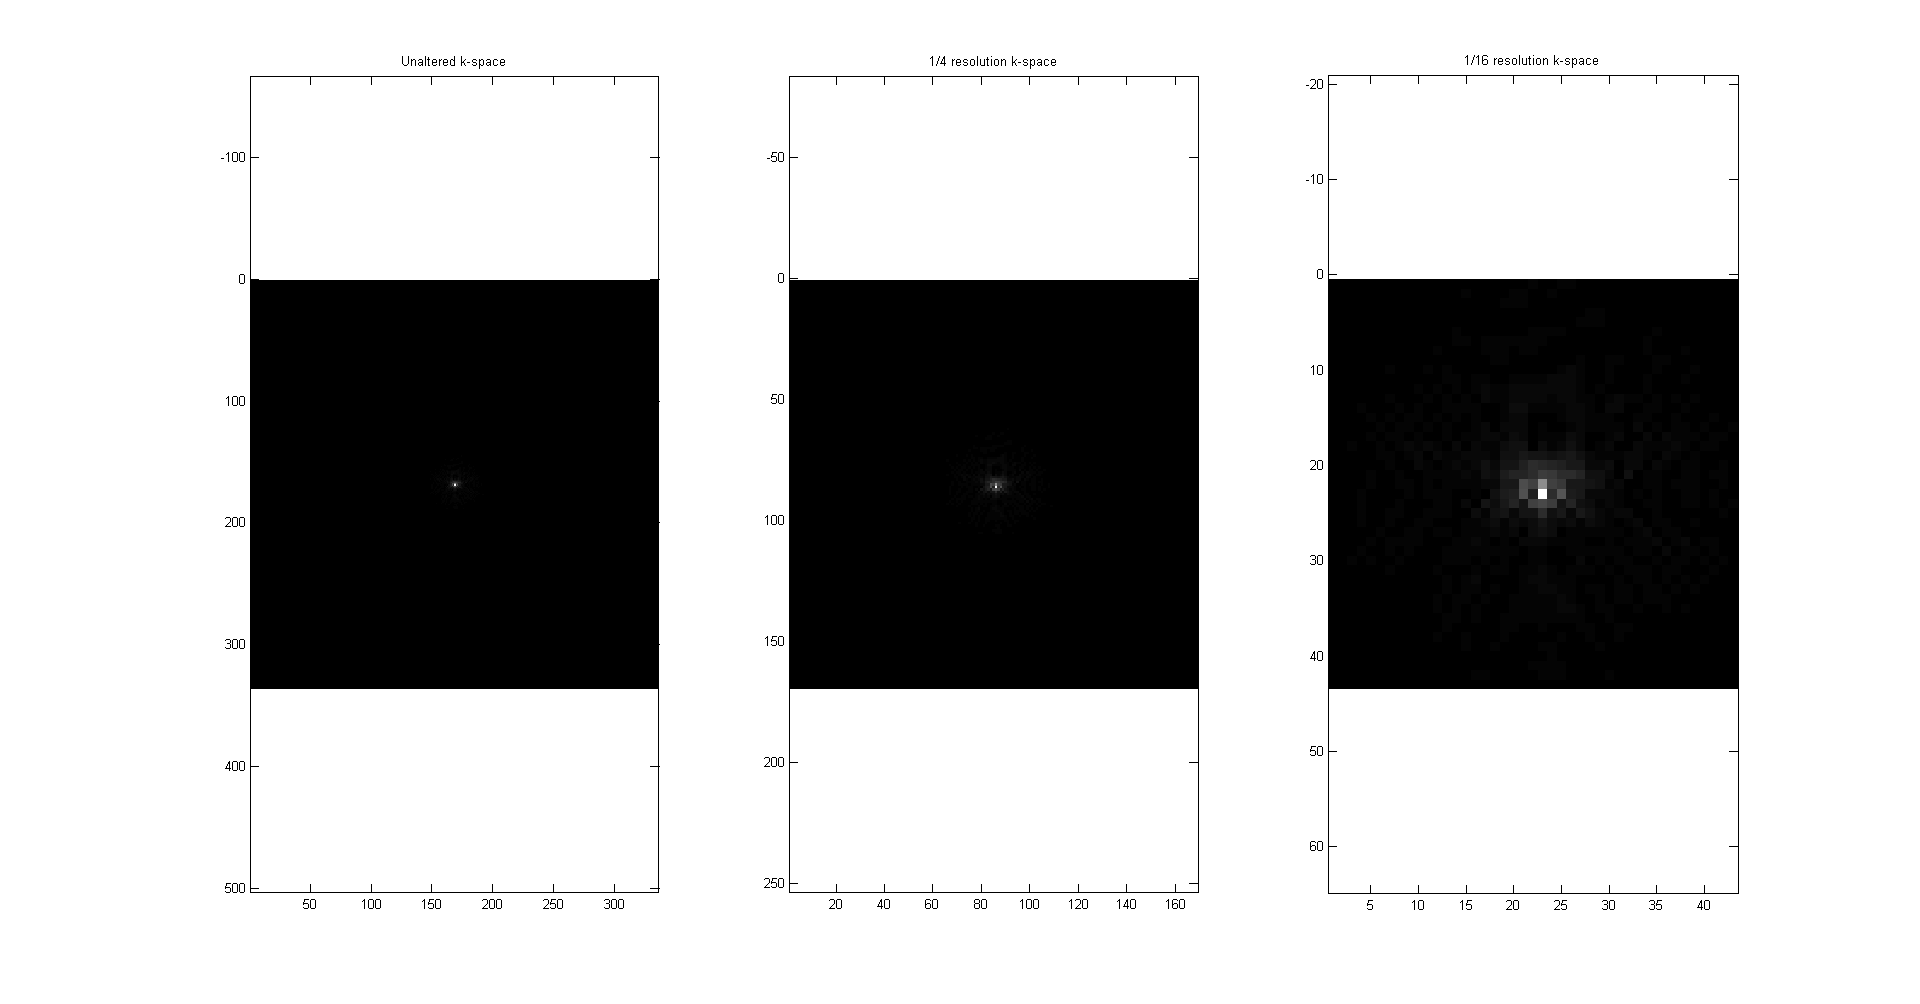
\includegraphics[width=\textwidth]{../images/KSpaceResolutions} \\
\newpage
\begin{lstlisting}   
brain = kspace2image(kspace); 
dims = size(brain);
mids = dims/2;

brain4 = brain(mids(1)-dims(1)/4:mids(1)+dims(1)/4, mids(2)-dims(2)/4:mids(2)+dims(2)/4);
brain16 = brain(mids(1)-dims(1)/16:mids(1)+dims(1)/16, mids(2)-dims(2)/16:mids(2)+dims(2)/16);

subplot(1,3,1);
imagesc(abs(brain));
title('Unaltered image');
axis equal;
colormap gray;
subplot(1,3,2);
imagesc(abs(brain4));
title('1/4 resolution image');
axis equal;
colormap gray;
subplot(1,3,3);
imagesc(abs(brain16));
title('1/16 resolution image');
axis equal;
colormap gray;

kspace4 = kspace(mids(1)-dims(1)/4:mids(1)+dims(1)/4, mids(2)-dims(2)/4:mids(2)+dims(2)/4);
kspace16 = kspace(mids(1)-dims(1)/16:mids(1)+dims(1)/16, mids(2)-dims(2)/16:mids(2)+dims(2)/16);
subplot(1,3,1);
imagesc(abs(kspace));
title('Unaltered k-space');
axis equal;
colormap gray;
subplot(1,3,2);
imagesc(abs(kspace4));
title('1/4 resolution k-space');
axis equal;
colormap gray;
subplot(1,3,3);
imagesc(abs(kspace16));
title('1/16 resolution k-space');
axis equal;
colormap gray;
\end{lstlisting}

\newpage

	\item[(d)]
		$\;$\\ 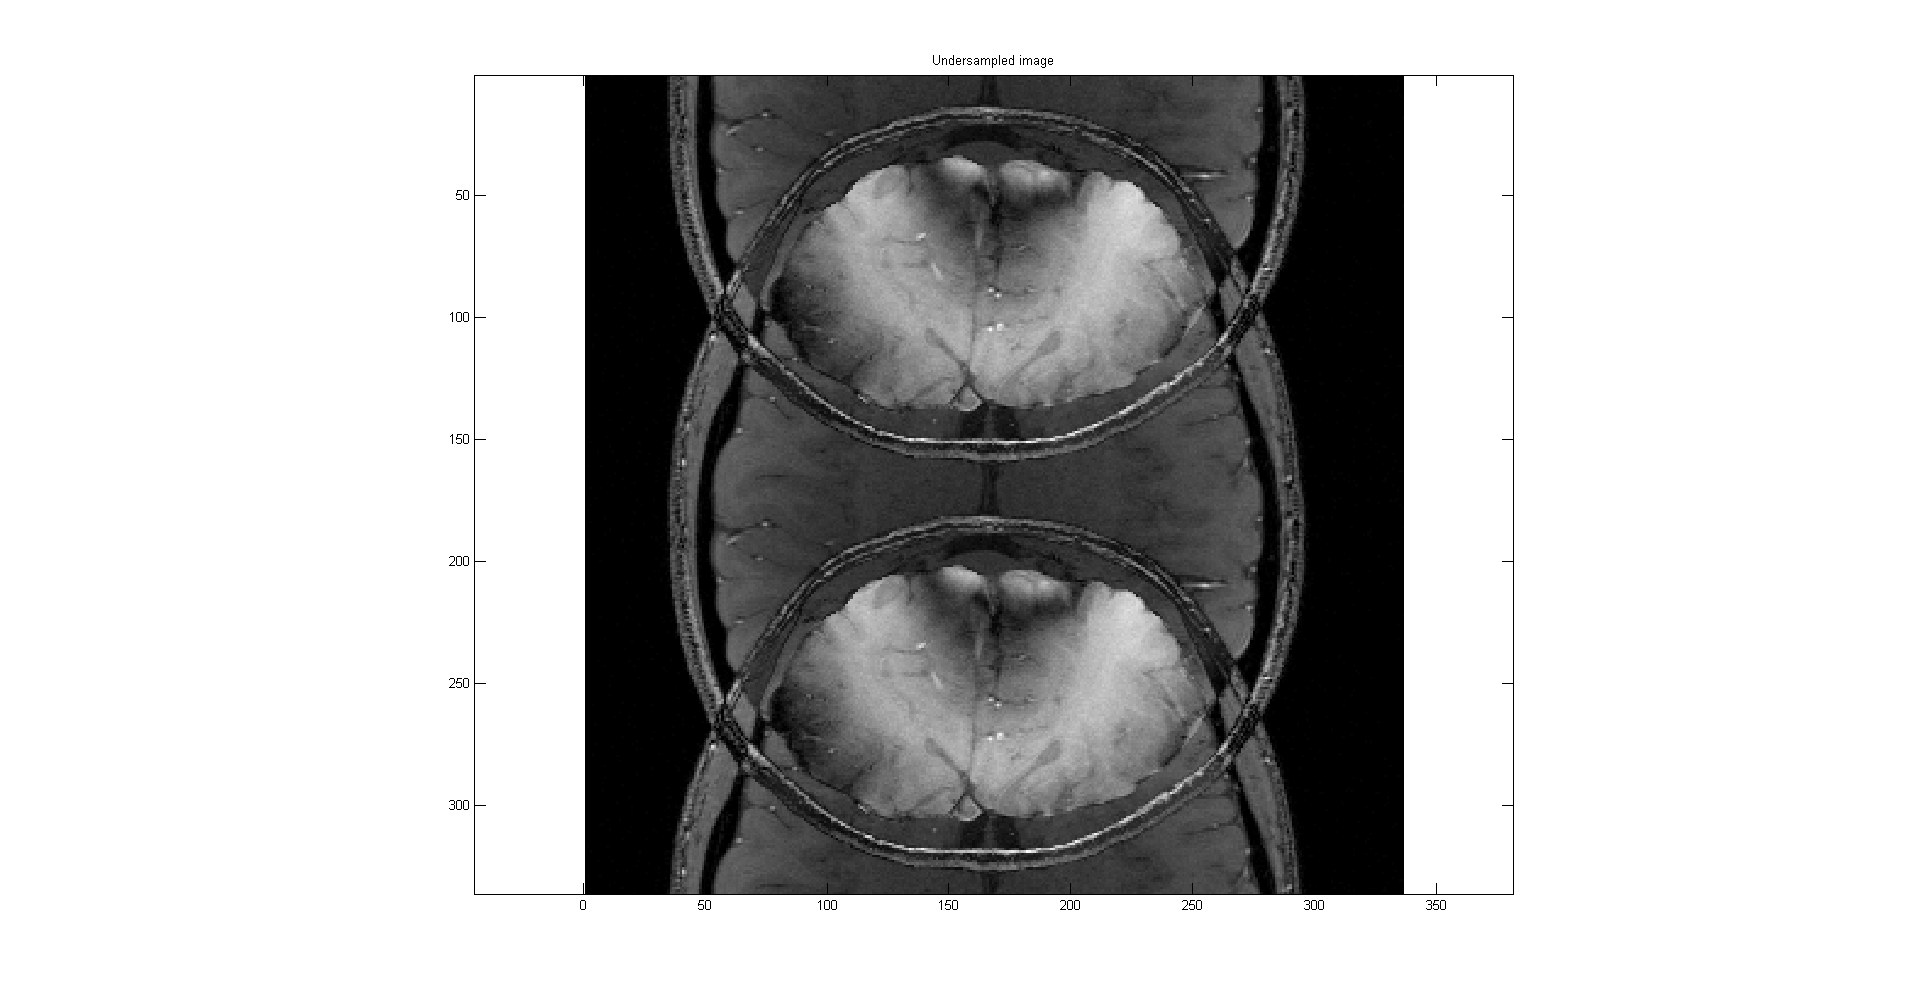
\includegraphics[width=\textwidth]{../images/BrainAliased} \\
\begin{lstlisting}   
kspace_undersampled = kspace;
kspace_undersampled(1:2:dims(1), :) = 0;
brain_undersampled = kspace2image(kspace_undersampled);
imagesc(abs(brain_undersampled));
title('Undersampled image');
axis equal;
colormap gray;
\end{lstlisting}
	\end{enumerate}

\newpage

\item[2.]
	\begin{enumerate}
	\item[(a)]
		The larger gradient caused a narrower width for the signals and a shift of each towards zero.\\
		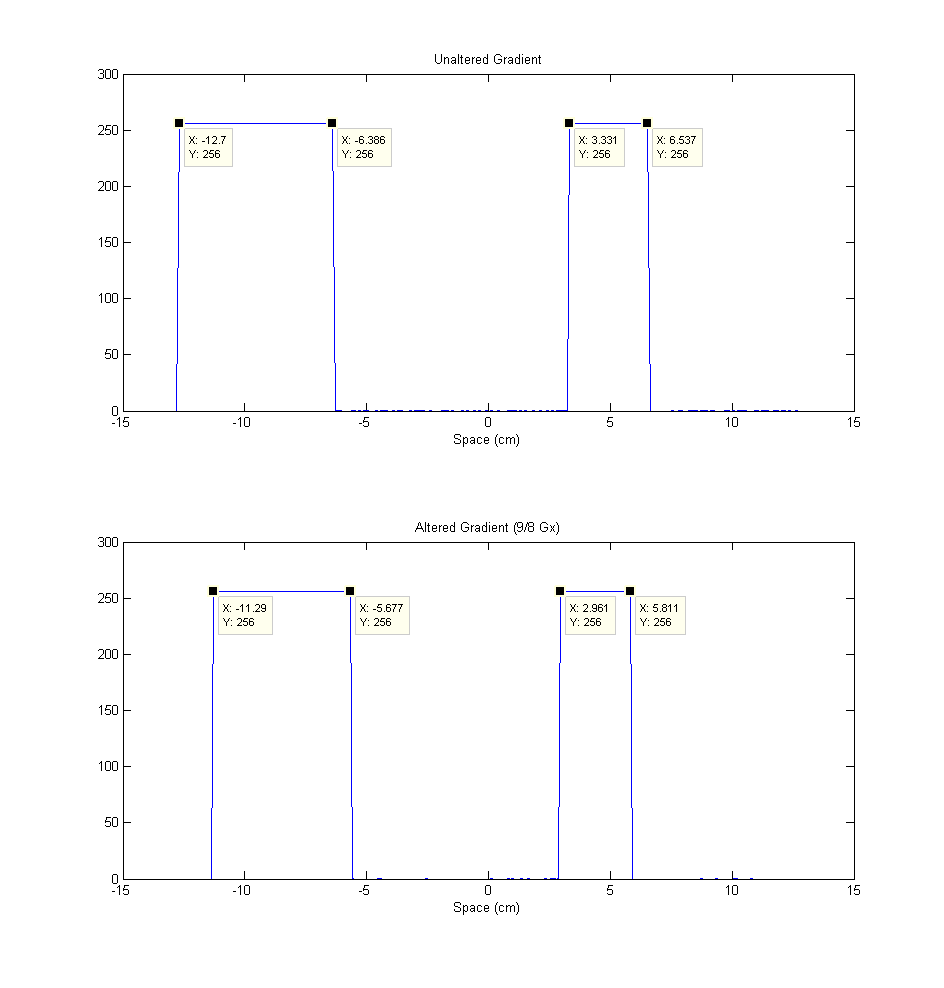
\includegraphics[width=\textwidth]{../images/AlteredGradient} \\
	\item[(b)]
		PLACE
\newpage
	\item[(c)]
		The negative gradient flips the signals about zero (compare to the first image of \texttt{(2a)}).\\
		\includegraphics[width=\linewidth]{../images/Negativegradient} \\
	\end{enumerate}

\end{enumerate}


\end{document}